\begin{figure}[htbp]
\section*{ ZNF462}
\centering
\begin{subfigure}[b]{0.95\textwidth}
\centering
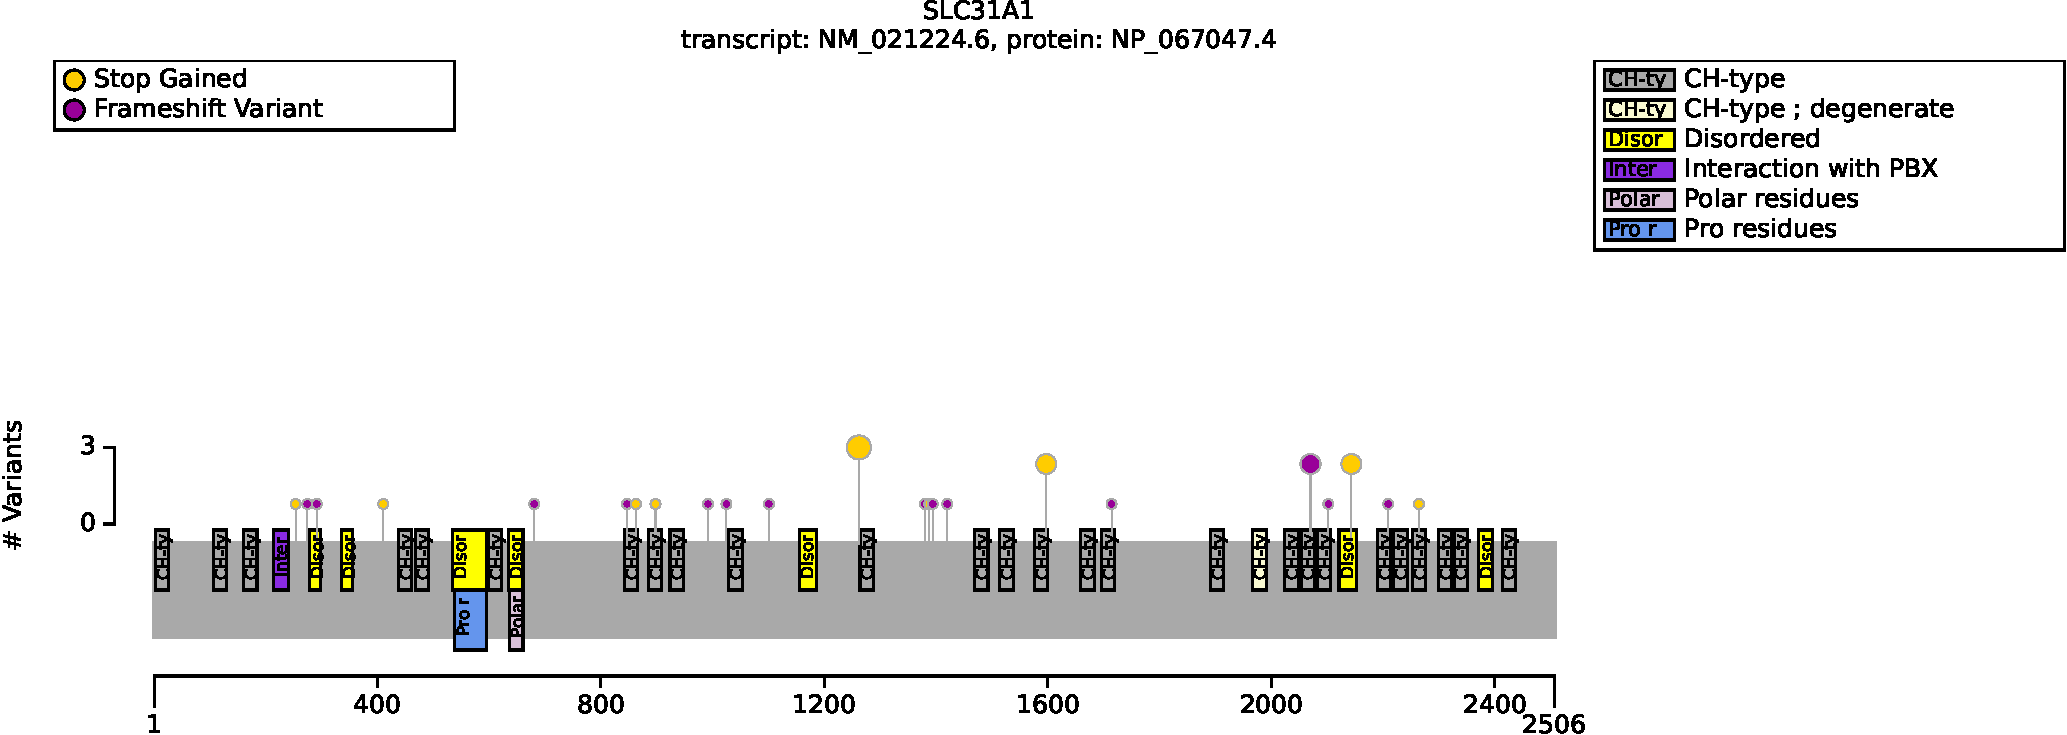
\includegraphics[width=\textwidth]{ img/ZNF462_protein_diagram.pdf} 
\captionsetup{justification=raggedright,singlelinecheck=false}
\caption{Distribution of variants in ZNF462}
\end{subfigure}

\vspace{2em}

\begin{subfigure}[b]{0.95\textwidth}
\centering
\resizebox{\textwidth}{!}{
\begin{tabular}{llllrr}
\toprule
Genotype (A) & Genotype (B) & total tests performed & significant results\\
\midrule
Ablation & Other & 43 & 0\\
FEMALE & MALE & 41 & 0\\
\bottomrule
\end{tabular}
}
\captionsetup{justification=raggedright,singlelinecheck=false}
\caption{Fisher Exact Test performed to compare HPO annotation frequency with respect to genotypes. }
\end{subfigure}

\vspace{2em}

\caption{ The cohort comprised 39 individuals (11 females, 25 males, 3 with unknown sex). 
A total of 32 HPO terms were used to annotate the cohort. Disease diagnosis: Weiss-Kruszka syndrome (OMIM:618619). 
No statistically significant genotype phenotype association was identified. 
A total of 26 unique variant alleles were found in \textit{ZNF462} (transcript: \texttt{NM\_021224.6}, protein id: \texttt{NP\_067047.4}).}
\end{figure}
